\begin{center}
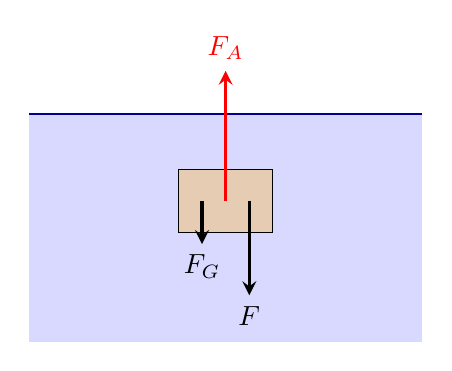
\begin{tikzpicture}[>=stealth]
 \fill[blue!15] (-2.5,-1.8) rectangle (2.5,1.1);
 \draw[blue!60!black, thick] (-2.5,1.1) -- (2.5,1.1);
 \draw[fill=brown!40] (-0.6,-0.4) rectangle (0.6,0.4);
 \draw[->, very thick, red] (0,0) -- (0,1.65) node[above] {$F_\text{A}$};
 \draw[->, very thick] (-0.3,0) -- (-0.3,-0.55) node[below] {$F_\text{G}$};
 \draw[->, very thick] (0.3,0) -- (0.3,-1.2) node[below] {$F$};
\end{tikzpicture}
\end{center}

Auf den Zapfen wirken der Auftrieb $F_\text{A} = \rho_\text{W}\,V\,g$ nach oben, die Gewichtskraft $F_\text{G} = \rho_\text{K}\,V\,g$ und die Druckkraft $F$ nach unten. Im Gleichgewicht ist
\begin{align}
 F_\text{A} &= F_\text{G} + F \quad\Rightarrow\quad \left(\rho_\text{W}-\rho_\text{K}\right)V\,g = F
\end{align}
Mit $\rho_\text{W} = \rhoWO$ und dem typischen Wert $\rho_\text{K} = \rhoKO$ für Kork (FoTaBe S.~187) folgt
\begin{align}
 V &= \VKoF \\
   &= \frac{\FD}{\left(\rhoW-\rhoK\right)\cdot\gE} \\
   &= \VKo \approx \result{\VKolP{0}{2}}
\end{align}
